\section{Overview of the dissertation}
This dissertation covers a variety of ways that nanophotonics can harness the physics of light, from manipulating optical forces at the nanoscale, to developing efficient ways to encode information in the architecture of light. The focus of the thesis will be to understand the optical forces that are generated on nanoparticles and demonstrate the applications of such forces. 

The first chapter of this thesis introduces the field of nanophotonics and explains how electron density waves that propagate along a metal-dielectric interface, commonly known as plasmons, can have such a large impact on the field. Following, is a brief introduction on how plasmonic excitations are born, as well as the forces that result from the high electric field density plasmons are known for.
In chapter 2 the development of magneto-optical responses in plasmonic materials, that explores the magnetization of nanoparticles via the illumination of circularly-polarized light. This phenomenon offers a new degree of control over the Lorentz force exerted on plasmonic nanoparticles. As described in the third chapter, Lorentz forces influence the motion of anisotropic nanoparticles, namely nanowires, illuminated at oblique incidences, and the non-intuitive motion subsequently results. The following chapter (chapter 4) illustrates an efficient way to spatially encode information with fractal architecture. Finally, in chapter 5 polarization properties are explored for a metasurface composed of non-chiral sub-structures, the phenomenon of which is derived from the Lorentz force that occurs between substructures that are measured in the polarization properties as light passes through the material.

As of recent, there has been a lot of interest in the development of 3D (metamaterials) and 2D (metasurface) geometries that possess optical properties not found in nature. While there has been much advancement in the field, such as the fabrication of negative index materials [\cite{Padilla:2006, Dolling:07, shelby:489}], perfect lenses [\cite{Khorasaninejad:2016, Yang:14, Khorasaninejad1190}], and materials with permittivity close to zero [\cite{JPark:2015c, Alu:07}], many of these materials are limited to a small sample area and possess other pitfalls of top-down processing. Complete understanding of the optical forces generated on metallic nanoparticles leads the way to facilitate bottom-up processing of metasurfaces and metamaterials suitable for large-scale production. 

Ultimately, it is hoped that this work furthers the research on how metasurfaces and metamaterials are designed, fabricated, and applied.
%\section{Light}

%\section{}
%The study of optical phenomena related to the electromagnetic response of metals,
%which is the topic of this work, led to the development of an emerging and fast
%growing research field called plasmonics.
\section{Light and Polarization}
Electromagnetic waves are derived from non-zero solutions of Maxwell’s equations in vacuum in absence of electric charges [\cite{jackson, Landau}]. Polarization refers to the direction of the electromagnetic field vectors in space. Like color or intensity, the polarization of an electromagnetic wave is a fundamental property. The polarization in the most general sense, can be described by elliptical motion, relating to the path the electric field vector follows as the wave propagates. There are many light-matter interactions that depend on the incident polarization of the incident light, for example the strength of reflections, absorption or scattering [\cite{Hulst}]. Following conventions, we can consider the electric field of an plane electromagnetic wave travelling in the $z$-direction in Cartesian coordinates ($x,y,z$):
\begin{equation}
\mathbf{E}(t, z) =\mathbf{E}_0 \cos(\omega t-kz-\phi),
\end{equation}where $\mathbf{E}_0$ is the magnitude of the electric field in the $x-y$ plane, $\omega$ is the angular frequency, $t$ refers to time, $k$ is the wave-vector, and $\phi$ denotes some arbitrary phase. The electric field vector is perpendicular to the direction of propagation, $z$, so we can decompose the electric fields into $x$ and $y$ components:
\begin{equation}
\begin{aligned}
E_x(t) = E_{x0} \cos(\omega t-kz-\phi_x),\\
E_y(t) = E_{y0} \cos(\omega t-kz-\phi_y),\\
\end{aligned}
\end{equation}
where $\phi_x$ and $\phi_y$ refer to the phase associated with the electric field in their respective direction. Special cases of elliptical polarization occur when $\phi_x = \phi_y$, referring to linear polarization, and $|\phi_x-\phi_y| = \pi/2$ refers to circular polarization.

%The use of the polarization to achieve additional functionality that cannot be realized with any other optical technology is an exciting prospect to be exploited. 
Traditionally, the polarization of light is manipulated through interaction with uniaxial or biaxial materials, such as calcite or quartz. However, if the light-matter interaction is understood fundamentally at the nanoscale, polarization-dependent interactions can be artificially crafted through the precise design of a structure. 

\section{Surface plasmon polaritons}

Plasmonics [\cite{Barnes}] – named after the electron density waves that propagate along a metal-dielectric interface is a blossoming sub-field of optics. In particular there has been a tremendous amount of progress in the fabrication and manipulation methods of nanometer-sized objects in the last few decades that has allowed us to make significant leaps and bounds in the field of optics. %Plasmonic excitations need specific environmental conditions  for excitation by photons including a polarization-dependence of the incident photons

Certain promises that the sub-field of plasmonics offers are responsible for the surge of interest in the research field, for example a new generation of ultra-fast computing [\cite{Atwater07}], new possibilities to treat cancer and HIV/AIDS [\cite{Kumar2011}], topological insulators [\cite{Deshko16}], or the ability fabricate negative-refraction materials and perfect lenses [\cite{Urbas2016}]. This could be made possible because plasmonics bridges the microscopic with the nanoscopic by confining light on sub-wavelength volumes. Plasmonic structures are typically composed of metallic nanostructures or thin-films interfacing with a dielectric medium, in particular noble metals are employed as their high electron density causes plasmonic excitation to occur in the visible regime.

\subsection{The Drude Model}

The Drude model [\cite{Drude:00}] is one intuitive way to represent the excitation of plasmons, that treats the motion of electrons as a free electron gas that oscillates in response to an external electromagnetic field with a characteristic damping rate, $\gamma$. The equation of motion can be written as:
\begin{equation}
m\ddot{\mathbf{r}}+m\gamma\dot{\mathbf{r}} = -e\mathbf{E},
\label{drude_eq1}
\end{equation}
where $m$ is the mass of the electron, $\mathbf{r}$ is the spatial position vector, dot formalism refers to derivatives with respect to time, $e$ is the charge on the electron, and $\mathbf{E}$ is the driving electric field. If we assume a time-harmonic response of the motion, $r(t) = r_0e^{-i\omega t}$, and a time-harmonic driving field of the same frequency, $E(t) = E_0e^{-i\omega t}$, an ansatz for the Eq.~\ref{drude_eq1} exists:
\begin{equation}
\mathbf{r}(t) = \frac{e}{m(\omega^2+i\gamma\omega)}\mathbf{E}(t)
\end{equation}
which describes the complex amplitude of the electron gas motion and incorporates any phase difference with the driving field. The macroscopic polarization varies from the displacement of electrons according to $\mathbf{P}=-ne\mathbf{r}$, where $n$ is the electron density of the material, such that:
\begin{equation}
\mathbf{P} = \frac{ne^2}{m(\omega^2+i\gamma\omega)}\mathbf{E}.
\end{equation}
Inserting this relation for the macroscopic polarization density into the relation for displacement field, $\mathbf{D}$ and electric field
\begin{equation}
\begin{split}
D &= \epsilon_0 E+P,\\
D &= \epsilon_0 \epsilon E.
\end{split}
\end{equation}
The relation for the displacement field then becomes:
\begin{equation}
D = \epsilon_0(1-\frac{\omega_p^2}{\omega^2+i\gamma\omega})E.
\end{equation}
where $\epsilon_0$ is the permittivity of free space, and $\omega_p$ is the plasma frequency such that $\omega_p = \sqrt{\frac{n^2e}{m\epsilon_0}}$.
The perittivity of the metal can then be written as:
\begin{equation}
\epsilon(\omega) = 1-\frac{\omega_p^2}{\omega^2+i\gamma\omega},
\end{equation}
where the real and imaginary parts of this complex function $\epsilon(\omega) = \epsilon_r(\omega)+i\epsilon_i(\omega)$ look as follows:
\begin{equation}
\begin{aligned}
\epsilon_r(\omega) = 1 - \frac{\omega_p^2}{\gamma^2+\omega^2}\\
\epsilon_i(\omega) = \frac{\omega_p^2\gamma}{\omega(\gamma^2+\omega^2)}
\end{aligned}
\end{equation}
The Drude model is sufficient in explaining the AC conductivity in metals, however it is insufficient at describing the optical properties of noble metals in the visible regime. By adding a spring-like resonance term to Eq.~\ref{drude_eq1} the model performs much better. In the visible portion of the electromagnetic spectrum, the frequency of electromagnetic waves coincide with the natural oscillation of free electrons in noble metals; when polarization-specific light is incident on noble metals the free electrons oscillate in resonance. 
\begin{equation}
m\ddot{\mathbf{r}}+m\gamma\dot{\mathbf{r}}-\omega_0^2 = -e\mathbf{E},
\label{drude_eq2}
\end{equation}

This leads to a Lorentz-oscillator form of the motion of the charge particle [\cite{Vial}], known as the Lorentz-Drude model where the complex permittivity becomes:
\begin{equation}
\begin{split}
\epsilon_r(\omega) &= 1-\frac{\omega_p^2}{\omega^2-\omega_0^2+\gamma^2}\\
\epsilon_i(\omega) &= \frac{\omega_p^2\gamma}{\omega(\omega^2-\omega_0^2+\gamma^2)}\\
\end{split}
\label{eps_m}
\end{equation}
The modified dielectric constant gives rise to a number of interesting properties that include a modification to the refractive index and conductivity of the material.

The dispersion relation for a plasma is given by the relation $\omega^2 = \omega_p^2+c^2k^2$ which results in an asymptotically linear behaviour. Figure~\ref{dispRelation} shows an example of the dispersion relation of aluminium.
\begin{figure}[b!]
\centering
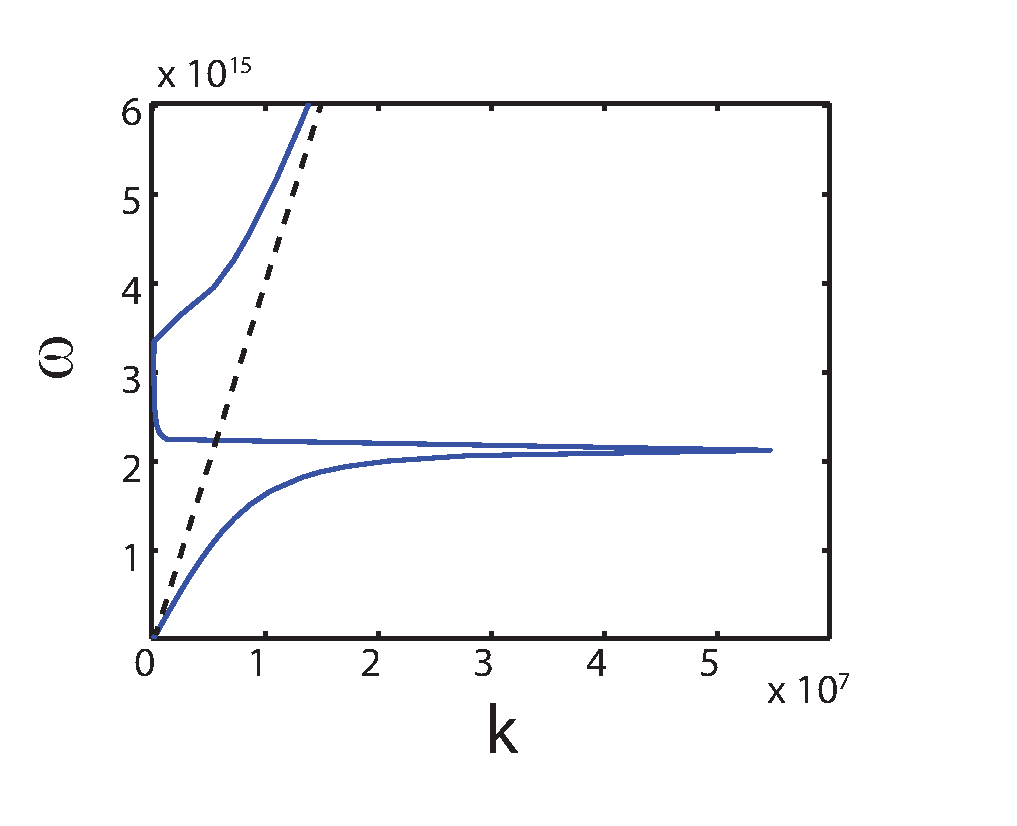
\includegraphics[width=0.75\textwidth]{dispRelation.pdf}
\caption{Dispersion relation of surface plasmon modes in aluminium with water ($\epsilon_d=1.77$) as the surrounding dielectric. Dashed line represents the light line.}
\label{dispRelation}
\end{figure}

Surface plasmon modes are oscillations of plasma, their properties can be derived from Maxwell's equations. Interestingly, when these equations are solved with the appropriate boundary conditions between a noble metal and a dielectric the surface plasmon mode produced can have a larger momentum than the free-space photon that produced it $(k_{SP}>k_0)$, where the frequency-dependent surface plasmon wave-vector is given by the relation [\cite{Sambles}]:
\begin{equation}
k_{SP} = k_0\sqrt{\frac{\epsilon_d\epsilon_m}{\epsilon_d+\epsilon_m}}
\label{ksp}
\end{equation}
where $\epsilon_d$ is the dielectric constant of the surrounding dielectric and $\epsilon_m$ is the dielectric constant of the metal calculated from Eq.~\ref{eps_m}. A detailed derivation of Eq.~\ref{ksp} is included in Section~\ref{deriv}. This leads to a dispersion relation as seen in Fig.~\ref{dispRelation}. The high wave vectors of surface plasmons lead to greatly-enhanced light-matter interactions [\cite{Todorov}].

In general mode-matching conditions are satisfied by either using a prism, or other dielectric with permittivity $\>$1, to couple light at the interface [\cite{Kretschmann}], through defects on the surface [\cite{Hecht}], or via diffraction with periodic surface structures such as gratings [\cite{Ritchie}].

Surface plasmons are known by two kinds, surface plasmon polaritons (SPPs) and localized surface plasmons (LSPs) [\cite{MaierBook}]. SPPs are composed of an electron density wave (plasmon part) coupled to a light wave (polariton part) and travel along the metal-dielectric interface. The dispersion relation dictates the wavelength  of the SPP, the coupling of light to the SPP results in a reduction of the free-space wavelength that is beneficial for electric field confinement. SPPs are commonly excited by 2D periodic grating structures as the periodic structure is able to provide the necessary in-plane wave-vector matching conditions. LSP resonances are a localized resonances of the charge density around nanostructures smaller than the wavelength of light. The resonance is highly dependent on the size, shape, material and surrounding environment of the nanostructure [\cite{Link1}], making them excellent candidates for sensors, in which small changes in environmental conditions are to be detected.

\subsection{Coupling to Plasmons}
\label{deriv}

The surface plasmon dispersion can be derived from first principles as follows. First, a TM excitation wave is considered travelling in the $x-z$ plane incident on a metal dielectric interface at $z=0$, in which $E_y = 0$, $H_x = H_z = 0$, where $E$ and $H$ represent the electric and magnetic fields respectively and subscripts denote the relative direction. From this the electric and magnetic fields in the metal and dielectric can be written:
\begin{equation}
\begin{pmatrix}
E_{xd} \\
0 \\
E_{zd}
\end{pmatrix} \exp[i(k_{xd}+k_{zd}-\omega t)],
\begin{pmatrix}
0\\
H_{yd} \\
0
\end{pmatrix} \exp[i(k_{xd}+k_{zd}-\omega t)];
\end{equation}
\begin{equation}
\begin{pmatrix}
E_{xm} \\
0 \\
E_{zm}
\end{pmatrix} \exp[i(k_{xm}+k_{zm}-\omega t)],
\begin{pmatrix}
0\\
H_{ym} \\
0
\end{pmatrix} \exp[i(k_{xm}+k_{zm}-\omega t)];
\end{equation}
where $k$ is the wave-vector, $\omega$ is the angular velocity and $t$ refers to time. The boundary conditions at the metal-dielectric interface are as follows:
\begin{equation}
\begin{split}
\epsilon_mE_{zm} &= \epsilon_dE_{zd}\\
E_{xm} &= E_{xd}\\
H_{ym} &= H_{yd}
\end{split}
\end{equation}
where $\epsilon$ refers to the dielectric constant. The last of the two boundary conditions lead to the equivalence of in-plane wave-vector, $k_x$:
\begin{equation}
k_{xm} = k_{xd}
\end{equation}
Solving Maxwell's equations, $\nabla\times \mathbf{H} = \frac{\epsilon}{c}\partial_t\mathbf{E}$:
\begin{equation}
\begin{pmatrix}\partial_x\\\partial_y\\\partial_z\end{pmatrix}\times
\begin{pmatrix}0\\H_y\\0\end{pmatrix} = \frac{\epsilon}{c}\partial_t
\begin{pmatrix}E_x\\0\\E_z\end{pmatrix}
\end{equation}
\begin{equation}
\begin{pmatrix}-\partial_zH_y\\0\\\partial_xH_y\end{pmatrix}
= \frac{\epsilon\omega}{c}
\begin{pmatrix}E_x\\0\\E_z\end{pmatrix}
\end{equation}
\begin{equation}
\begin{split}
(I): -k_{zm}H_ym &= \frac{\epsilon_m\omega}{c}E_xm \\
(II): k_{zd}H_yd &= \frac{\epsilon_d\omega}{c}E_xd \\
(I)/(II): \frac{k_{zm}}{k_{zd}}\frac{H_{ym}}{H_{yd}} &=-\frac{\epsilon_m}{\epsilon_d}\frac{E_{xm}}{E_{xd}},
\end{split}
\end{equation}
where region $(I)$ represents the metal and region $(II)$ represents the dielectric. Using the boundary condition $E_{xm} = E_{xd}$ and $H_{ym} = H_{yd}$ and the general relation $k_x^2+k_y^2+k_z^2 = k^2 = \epsilon\frac{\omega^2}{c^2}$
The relations for the in and out-of-plane vectors are obtained:
\begin{equation}
\begin{split}
k_x^2 &= \frac{\omega^2}{c^2}\frac{\epsilon_m\epsilon_d}{\epsilon_m+\epsilon_d}\\
k_zm^2 &= \frac{\omega^2}{c^2}\frac{\epsilon_m}{\epsilon_m+\epsilon_d}\\
k_zd^2 &= \frac{\omega^2}{c^2}\frac{\epsilon_d}{\epsilon_m+\epsilon_d}\\
\end{split}
\end{equation}
\begin{figure}[t!]
\centering
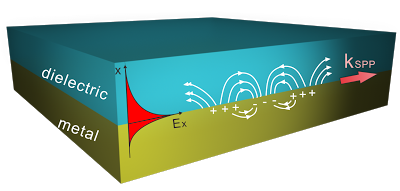
\includegraphics[width=0.95\textwidth]{SPP.png}
\caption{Surface plasmon polariton at a dielectric-metal interface. https://sites.google.com/site/caltechhowardlee/Research}
\end{figure}
%https://sites.google.com/site/caltechhowardlee/Research

\subsection{Nonlinear plasmonics}
\par Nonlinear effects are governed by photon-photon interactions in materials, and thus, are generally weak. The scattering and absorption cross-sections of plasmonic nanoparticles are much greater than their geometrical cross-sections which lead to large local field enhancements around the the nanostructures to enable nonlinear effects to occur. Due to high local field enhancement plasmonic excitations has enabled nonlinear phenomenon such as surface-enhanced Raman scattering [\cite{Nie}], second harmonic generation [\cite{Canfield}], and enhanced magneto-optical effects [\cite{Moocarme2014,Belotelov}]. A material's response to an electric field, $E$, is governed by the material polarization $P$ [\cite{Kauranen}]:
\begin{equation}
P = \epsilon_0\big[\chi^{(1)}E+\chi^{(2)}E^2+\chi^{(3)}E^3+\ldots\big]
\label{Pol}
\end{equation}
where $\chi^{(n)}$ is the $n$-th order susceptibility of the material [\cite{Boyd}]. In general the lower-order terms of Eq. \ref{Pol} dominate, however, in the presence of high electric fields, such as the fields generated by plasmonic resonances, the higher-order terms become non-negligible. The first order responses consistent with the $\chi^{(1)}$ term such as scattering and absorption have been studied for centuries and are well understood [\cite{Mie, Hulst}]. Optical responses of materials are less understood in the presence of strong electrics fields,  where nonlinear effects need to be considered. Frequencies of radiation different from the incident will be produced due to the $E^n$ term when $n\neq 1$. Moreover, these new frequencies may interact with the incident field that further influence the nonlinear fields produced. Sum- and difference-frequency generation are a result of the nonlinear response; an example of sum-frequency generation is two incident photons with the same frequency interact in the second order and produce one photon with double the frequency [\cite{Canfield}].

For a frequency $\omega$, first order responses vary as $\Re[e^{-i\omega t}]$; second order responses vary as $\Re[e^{-i\omega t}]^2 = \frac{1}{2}(1+\Re[e^{-2i\omega t}])$, where $\Re$ denotes the real part. This is where the similarity between the second order responses that oscillate $\propto 2\omega$ and the non-oscillating rectification responses are seen [\cite{Shen}]. To this end, DC responses will have the same magnitude  as the second harmonic, $\cos(2\omega t)$, term. It is these DC responses that are responsible for the Lorentz forces studied in this thesis. DC responses have nonzero time-averaged value where time-harmonic terms are zero, that allow DC responses to be easily measurable over their second-harmonic oscillating counterpart, especially at visible frequencies.

\section{Radiation and polarization forces}
The DC force on a particle in the presence of electromagnetic fields can be determined from the Lorentz force, $\mathbf{F}$ [\cite{Gordon}]:
\begin{equation}
\mathbf{F} = (\mathbf{p}\cdot\nabla)\mathbf{E}+\frac{1}{c}\frac{d\mathbf{p}}{dt}\times \mathbf{B},
\label{force1}
\end{equation}
where $\mathbf{p}$ is the dipole moment of the atom, $c$ is the speed of light, $\mathbf{E}$ is the electric field and $\mathbf{B}$ is the magnetic. The electric, magnetic field, and dipole moment vary time-harmonically such that $\mathbf{E} = \Re[\mathbf{E_0}e^{-i\omega t}]$, $\mathbf{B} = \Re[\mathbf{B_0}e^{-i\omega t}]$, $\mathbf{p} = \Re[\mathbf{p_0}e^{-i\omega t}]$. The time-average of the total force can be written as [\cite{Chaumet}]:
\begin{equation}
\langle \mathbf{F}\rangle = \frac{1}{4T}\int_{-T/2}^{T/2}\big[(\mathbf{p}+\mathbf{p}^*)\cdot\nabla(\mathbf{E}+\mathbf{E}^*)+\frac{1}{c}(\dot{\mathbf{p}}+\dot{\mathbf{p}}^*)\times(\mathbf{B}+\mathbf{B}^*)\big]dt,
\label{timeAv}
\end{equation}
where $\dot{\mathbf{p}} = d\mathbf{p}/dt$. Performing the integral of Eq.~\ref{timeAv} for the $i$th Cartesian component the time averaged force becomes:
\begin{equation}
\langle F^i\rangle = \frac{1}{2}\big[p_{0j}\partial^j(E_0^i)^*+\frac{1}{c}\epsilon^{ijk}\dot{p_{0j}}(B_{0k})^*\big],
\label{timeAv2}
\end{equation}
where $\epsilon^{ijk}$ is the Levi-Cevita symbol. The dipole moment can be written as a reaction to the electric field $\mathbf{p}=\alpha \mathbf{E}$, and using the Maxwell equation:
\begin{equation}
\nabla\times \mathbf{E} = \frac{1}{c}\frac{\partial \mathbf{B}}{\partial t} = \frac{-i\omega}{c}\mathbf{B}
\end{equation}
Equation \ref{timeAv2} then becomes:
\begin{equation}
\langle F^i\rangle =\frac{\alpha}{2}[E_{0j}\partial^j(E^i_0)^*+\epsilon^{ijk}\epsilon_{klm}E_{0j}\partial^l(E_0^m)^*]
\end{equation}
Using the relation between Levi-Cevita notation $\epsilon^{ijk}\epsilon_{klm} = \delta^i_l\delta^j_m-\delta_m^i\delta_l^j$ the time-averaged DC force can be written as:
\begin{equation}
\langle F^i\rangle = \frac{\alpha}{2}E_{0j}\partial^i(E_0^j)^*
\end{equation}
\begin{equation}
\langle \mathbf{F}\rangle = \frac{\alpha }{2}\sum_i E_i\nabla E_i^*
\label{Favg}
\end{equation}
Splitting Eq.~\ref{Favg} into real and imaginary components, the real part becomes:
\begin{equation}
\frac{\alpha}{2}\Re[\sum_i E_i\nabla E_i^*] = \frac{\alpha}{4}\Re[\nabla |\mathbf{E}|^2] = \frac{\alpha}{4}\nabla |\mathbf{E}|^2
\end{equation}
Which is commonly referred to as the gradient force [\cite{Ashkin:86, Proscia}]. Using vector identity product rules the imaginary component can be written as:
\begin{equation}
\frac{\alpha}{2}\Im[\sum_i E_i\nabla E_i^*] = \frac{\alpha}{2}\Im[\nabla\times\mathbf{E}\times\mathbf{E}^* + (\nabla\cdot\mathbf{E})\mathbf{E}^* + c.c.]
\end{equation}
This component is commonly referred to as the scattering force [\cite{KurosawaSPDE, Proscia}]. Both real and imaginary components contribute to the DC force from an oscillating electromagnetic field, the amount of each depend on the specific excitation conditions such as angle of incidence.
%
%\section{Decomposition of Poynting Vector}
%John Poynting more than a century ago that light carries momentum. He also showed that light carries angular momentum also, and that both properties of electromagnetic waves should be conserved in the quantum-mechanical nature of photons. In this section the the properties of the optical angular momentum are decomposed into spin and orbital angular momentum components [~\cite{Bliokh2014}].
%
%The momentum density $\vec{p}(r)$ of a quantum or classical wave field appears in the energy-momentum tensor within the corresponding field theory [\cite{Soper}], where momentum density also represents the energy flux density. For scalar fields, the momentum density can be written as a local expectation value of the canonical momentum operator$\hat{p} = -i\nabla$, \textit{i.e.},$\textbf{p} = \Re(\psi^\dagger\hat{p}\psi)$ where $\psi(r)$ is the wave function, and we use units : $\hbar =$ 1. However, for vector fields, an additional spin momentum density was introduced in 1939 by F.J. Belinfante [\cite{Belinfante}] to explain the spin of quantum particles and symmetrize the canonical energy-momentum tensor in field theory. 
%The optical momentum can be written as the sum of spin momentum component and a canonical (or orbital) momentum density, resulting in [\cite{Soper,Belinfante}]
%\begin{equation}
%\textbf{p} = \Re(\vec{\psi}^\dagger\hat{p}\vec{\psi})+\frac{1}{2}\nabla\times \textbf{s} \equiv \textbf{p}^O + \textbf{p}^S
%\label{AM1}
%\end{equation}
%Here $\vec{\psi}(r)$ is the spinor wave function, whereas s(r) is the spin angular momentum density. Equation \ref{AM1} are fundamental and hold true for various particles. In the case of photons, equation \ref{AM1} yields the time-averaged Poynting vector $\textbf{p} \propto k \Re(\textbf{E}\times \textbf{H}^*)$. Explicitly, the optical momentum and spin densities \ref{AM1} read:
%\begin{equation}
%\begin{aligned}
%\textbf{p}^O &= \frac{\gamma}{2}\Im[\textbf{E}^*\cdot\nabla\textbf{E}+\textbf{H}^*\cdot\nabla\textbf{H}]\\
%\textbf{p}^S &= \frac{1}{2}\nabla\times\textbf{s}\\
%\textbf{s} &= \frac{\gamma}{2} \Im[\textbf{E}\times \textbf{E}^* + \textbf{H}\times \textbf{H}^*]
%\end{aligned}
%\label{mom1}
%\end{equation}
%These quantities can be decomposed into electric and
%magnetic field contributions: $\textbf{p}^O = \textbf{p}^O_e + \textbf{p}^O_m$ and $\textbf{s}^O = \textbf{s}_e + \textbf{s}_m$. Though the Poynting vector \textbf{p} is usually considered in optics as a single momentum density of light, we can represent it as the sum of two quantities $\textbf{p}^O$ and $\textbf{p}^S$, that have different physical meanings and properties.
%
%The spin momentum density ($\textbf{p}^s$) can be thought of as the boundary magnetization current, whereas the spin angular momentum density ($\textbf{s}$) can be thought of as the bulk magnetization. The orbital momentum density, ($\textbf{p}^O$), contains the gradient of the electric field, and can be thought of as the term that is responsible for radiation pressure and energy transport. The spin momentum density term, ($\textbf{p}^s$), however, includes the term $\nabla\times\textbf{E}\times\textbf{E}^*$ and is the term generates the spin angular momentum of light [\cite{Bekshaev2011}].
%
